\documentclass[a4paper,12pt]{report}
\title{Tugas Data base II}
\author{Rayhan Yuda Lesmana}
\date{2 November 2019}
\usepackage{graphicx}

\begin{document}
\maketitle

\chapter{Tutorial}

\section*{Membuat workspace}
\begin{enumerate}

\item 
Masuk  ke website oracle Apex, lalu klik sign in.
\begin{figure}[h]

\includegraphics[width=4cm]{gambar/1.png}
\end{figure}

\item
Lalu click bacaan request a workspace,untuk membuat workspace baru.
\begin{figure}[h]
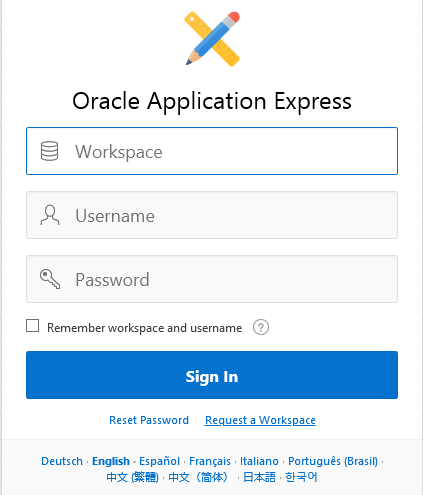
\includegraphics[width=4cm]{gambar/2.png}
\end{figure}

\newpage
\item
Lalu isi form yang sudah disediakan, setelah itu click next.
\begin{figure}[h]
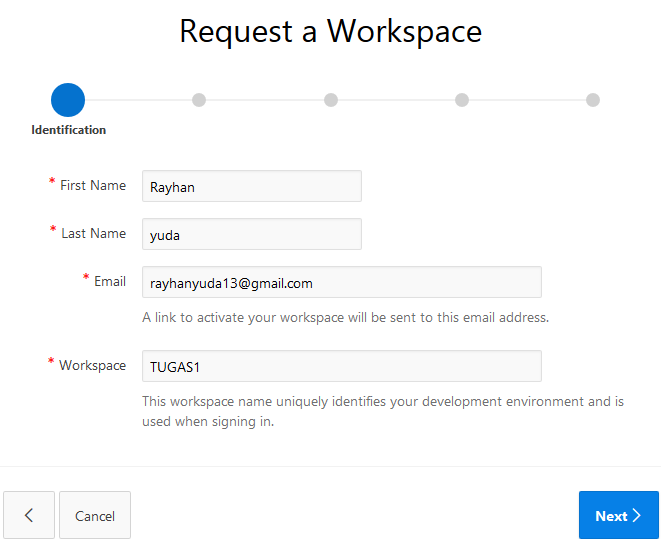
\includegraphics[width=3cm]{gambar/3.png}
\end{figure}

\item
Lalu isis survey yang di sediakan oleh oracle. Lalu click next
\begin{figure}[h]
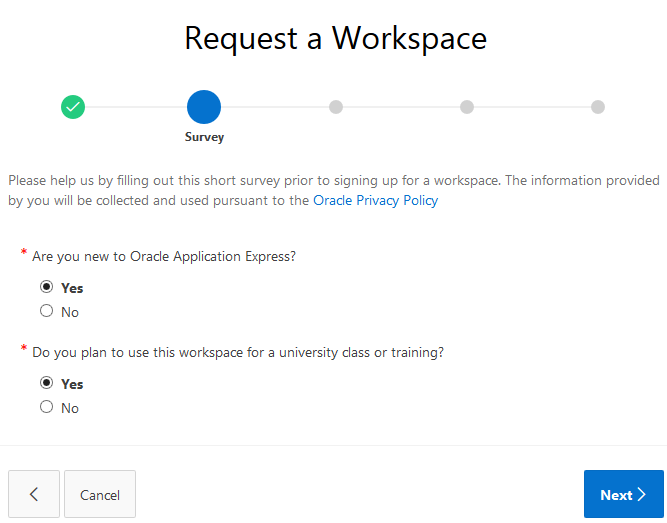
\includegraphics[width=3cm]{gambar/4.png}
\end{figure}

\item
isi pernyataan yang disediakan oleh oracle. Lalu click next.
\begin{figure}[h]
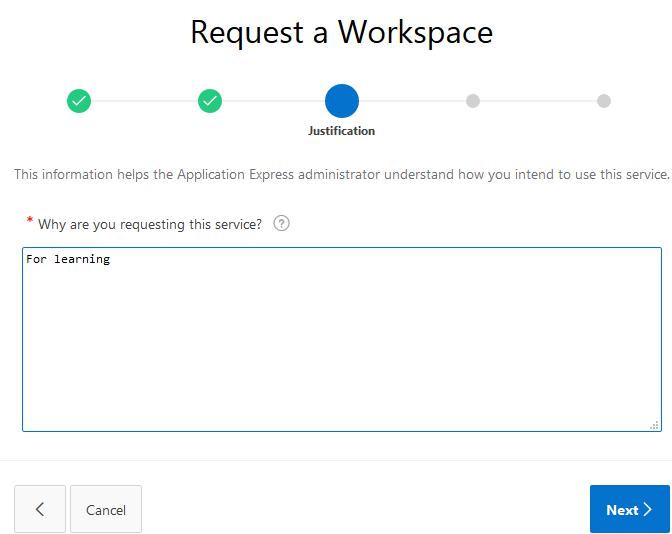
\includegraphics[width=4cm]{gambar/5.png}
\end{figure}

\newpage
\item
Lalu centang yang ada bacaan i accept the terms. Lalu click next.
\begin{figure}[h]
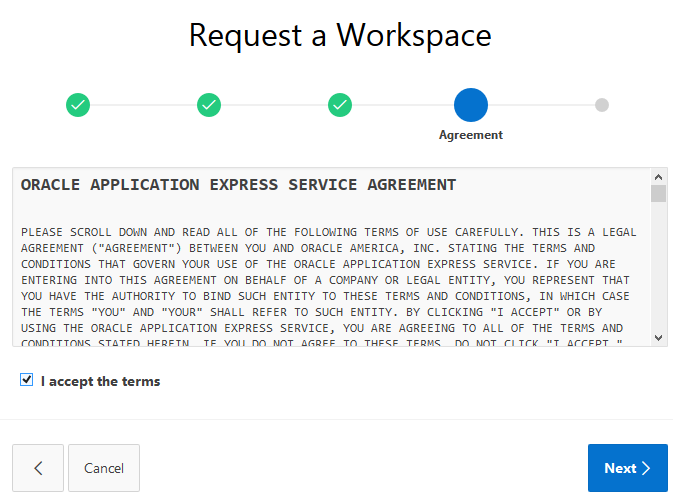
\includegraphics[width=4cm]{gambar/6.png}
\end{figure}


\item
Lalu click submit request.
\begin{figure}[h]
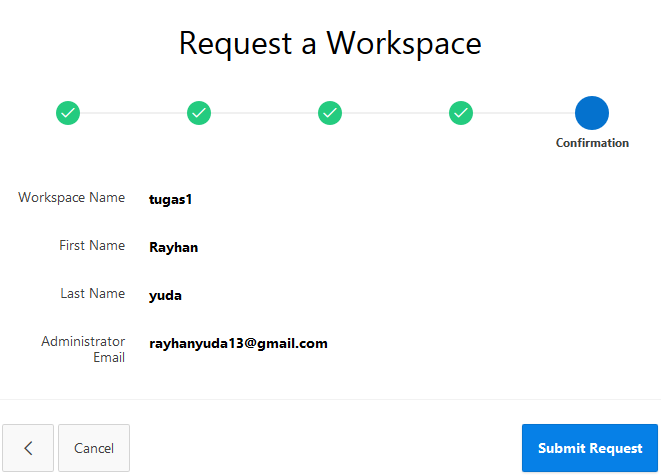
\includegraphics[width=4cm]{gambar/7.png}
\end{figure}

\item 
Lalu menunggu Email dari oracle nya.
\begin{figure}[h]
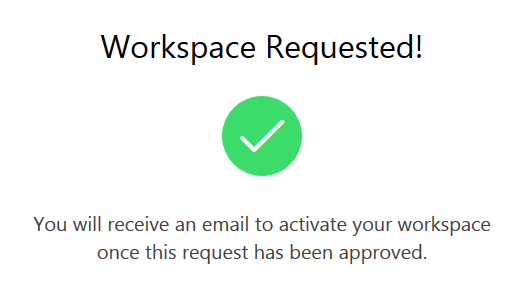
\includegraphics[width=4cm]{gambar/8.png}
\end{figure}

\newpage
\item
Setelah itu buka gmail anda, lalu click create workspace.
\begin{figure}[h]
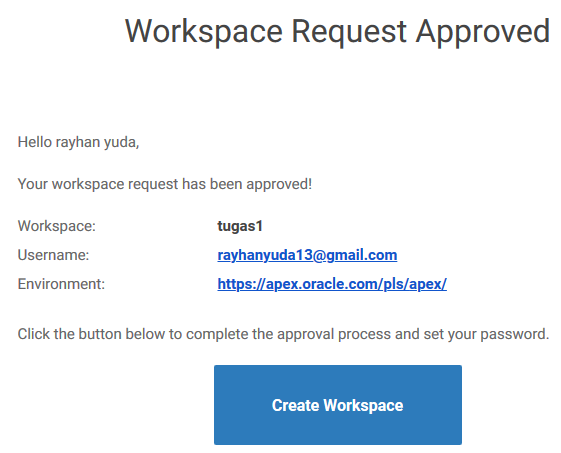
\includegraphics[width=4cm]{gambar/9.png}
\end{figure}

\item 
Lalu click continue to sign screen.
\begin{figure}[h]
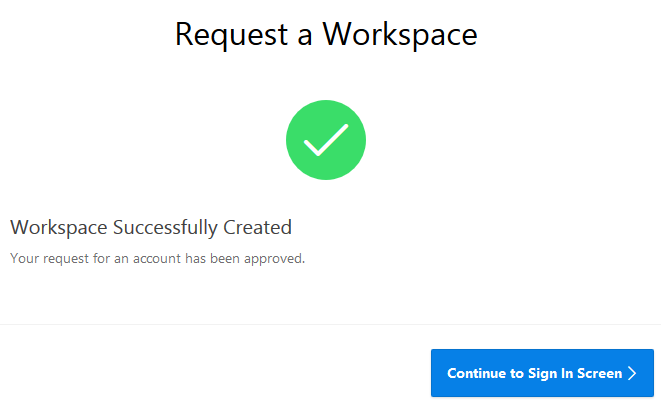
\includegraphics[width=4cm]{gambar/10.png}
\end{figure}

\item
Konfirmasi password email nya.
\begin{figure}[h]
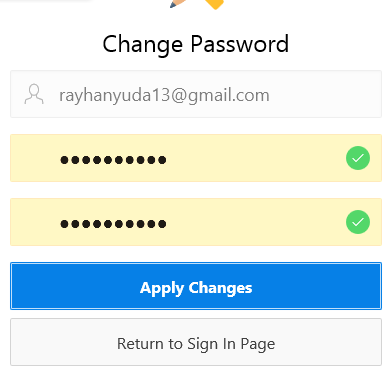
\includegraphics[width=4cm]{gambar/11.png}
\end{figure} 

\end{enumerate}

\chapter*{Membuat aplikasi}

\begin{enumerate}

\item
Click App builder.
\begin{figure}[h]
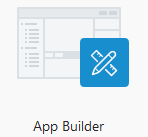
\includegraphics[width=4cm]{gambar/12.png}
\end{figure}

\item
Lalu click Create.
\begin{figure}[h]
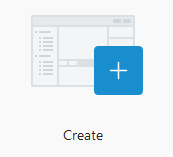
\includegraphics[width=4cm]{gambar/13.png}
\end{figure} 

\newpage 
\item
Lalu pilih From a file, Karena saya menggunakan File CVS sebagai data nya.
\begin{figure}[h]
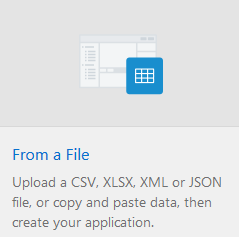
\includegraphics[width=4cm]{gambar/14.png}
\end{figure}

\item
Lalu drop file Cvs nya.
\begin{figure}[h]
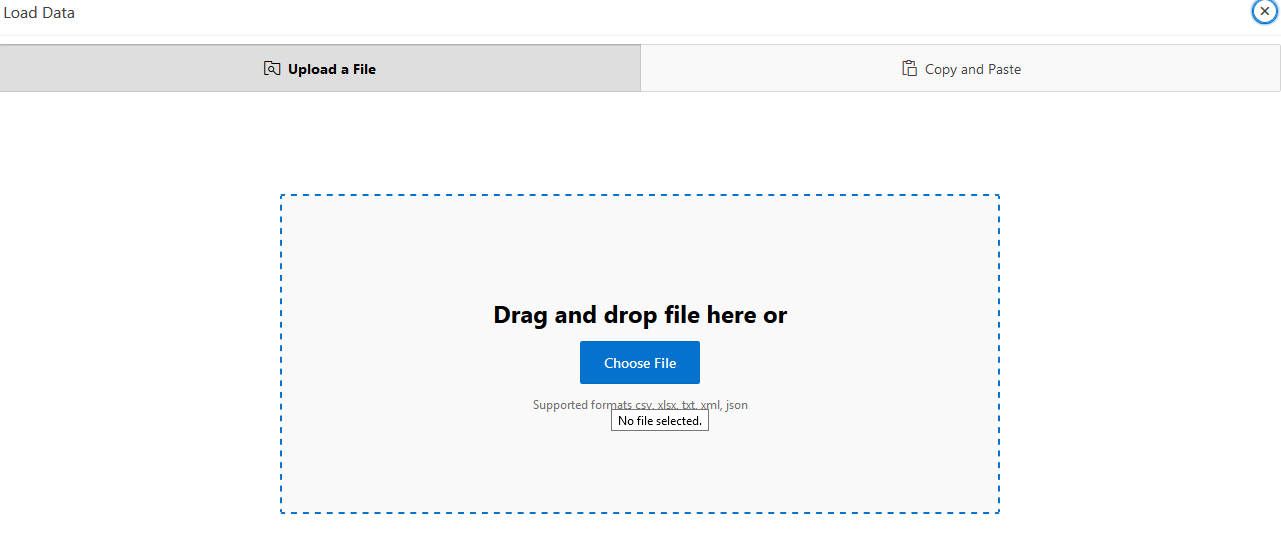
\includegraphics[width=4cm]{gambar/15.png}
\end{figure} 

\item
Lalu isi form yang telah di sediakan.
\begin{figure}[h]
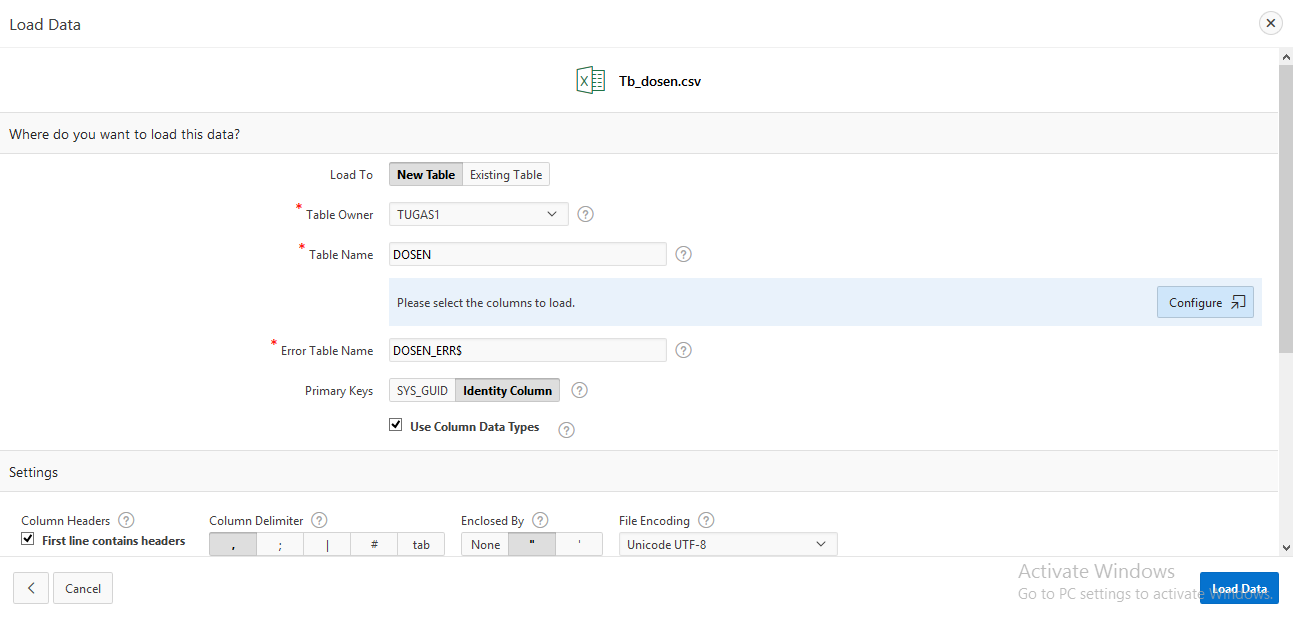
\includegraphics[width=4cm]{gambar/16.png}
\end{figure}

\newpage
\item
Configure Untuk memilih colums yang akan di load ke aplikasi, lalu click save changes, dan load data.
\begin{figure}[h]
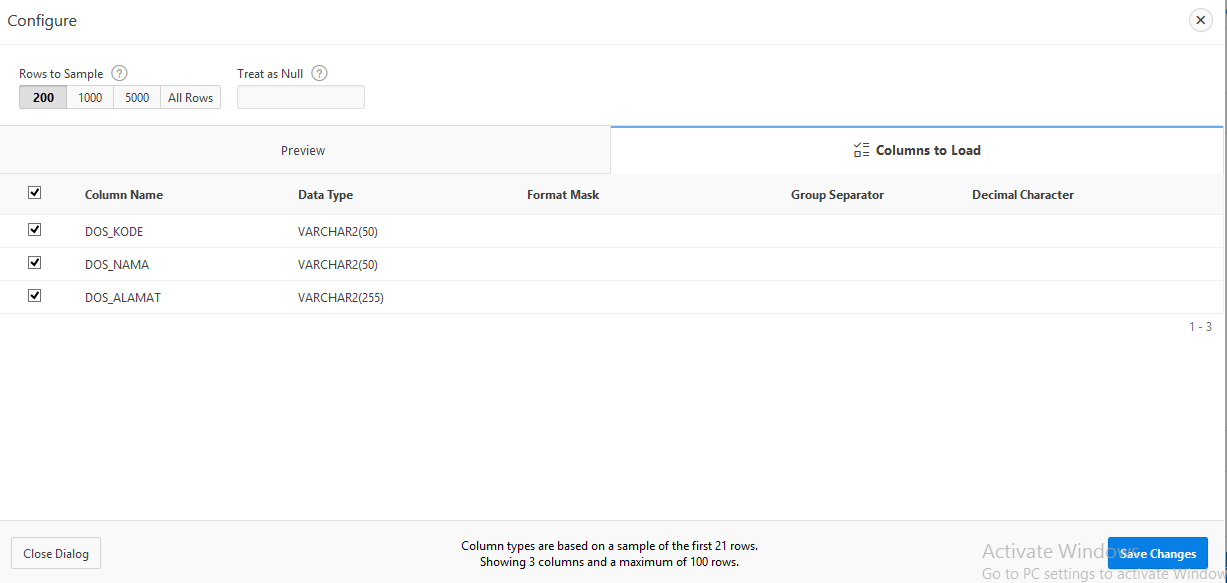
\includegraphics[width=4cm]{gambar/17.png}
\end{figure} 
 
\item
Lalu click create Application.
 \begin{figure}[h]
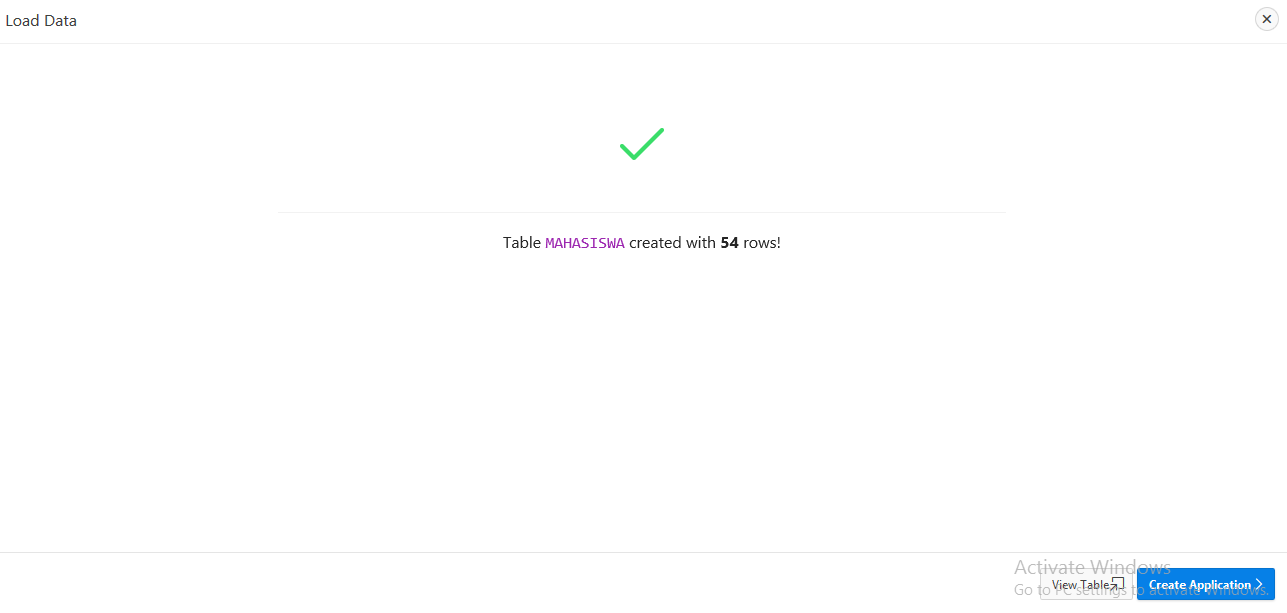
\includegraphics[width=4cm]{gambar/18.png}
\end{figure} 

\newpage
\item
add page untuk menambah table yang telah di load.
\begin{figure}[h]
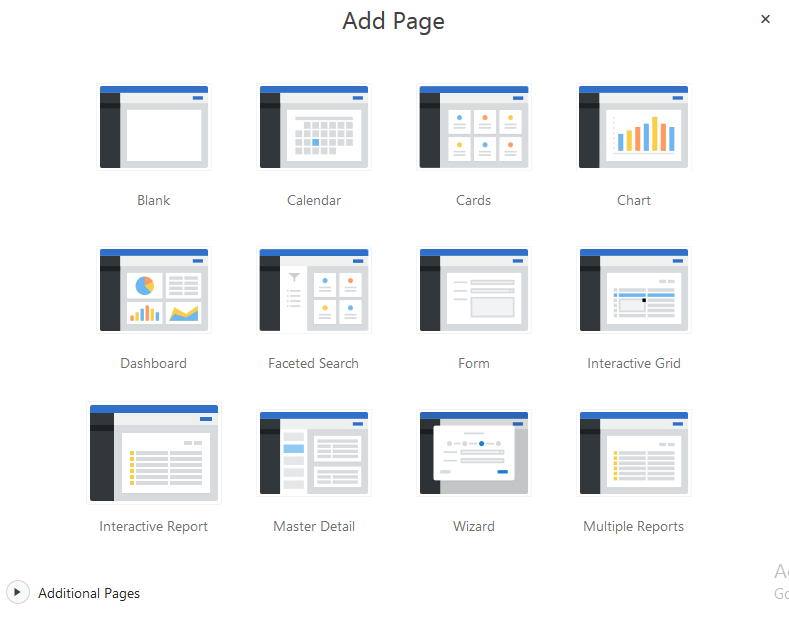
\includegraphics[width=4cm]{gambar/19.png}
\end{figure}

\item 
Page name : untuk mengisi nama yang akan di tampilkan di aplikasi.\\
Tabel or view : Memilih tabel yang akan di masukan.\\
Lalu click add page. 
\begin{figure}[h]
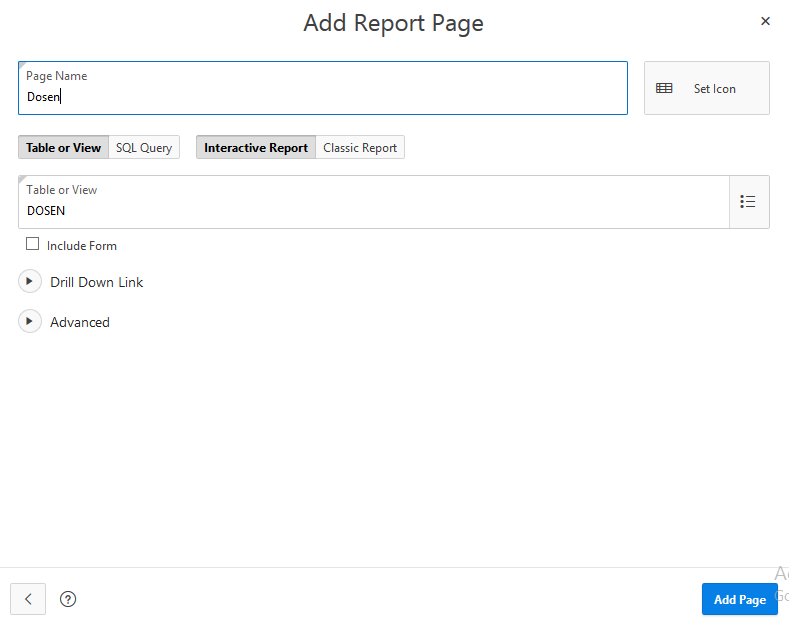
\includegraphics[width=4cm]{gambar/20.png}
\end{figure} 

\item
Lalu bacaan create application untuk membuat aplikasi nya.
\begin{figure}[h]
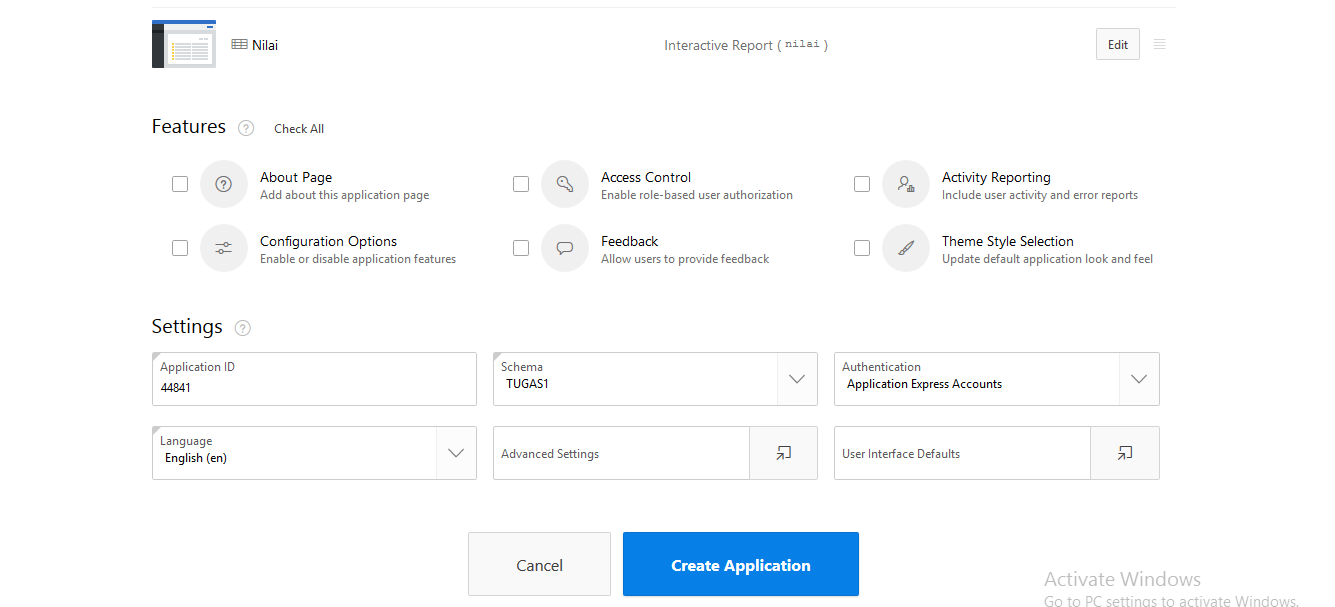
\includegraphics[width=4cm]{gambar/21.png}
\end{figure} 

\newpage
\item
Lalu click bacaan run item.
\begin{figure}[h]
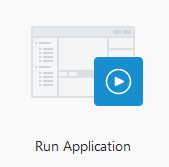
\includegraphics[width=4cm]{gambar/22.png}
\end{figure} 

\item
Lalu sign in menggunakan email.
\begin{figure}[h]
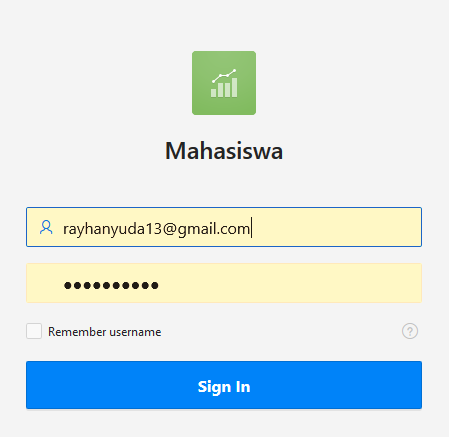
\includegraphics[width=4cm]{gambar/23.png}
\end{figure}

\item
Aplikasi telah di buat
\begin{figure}[h]
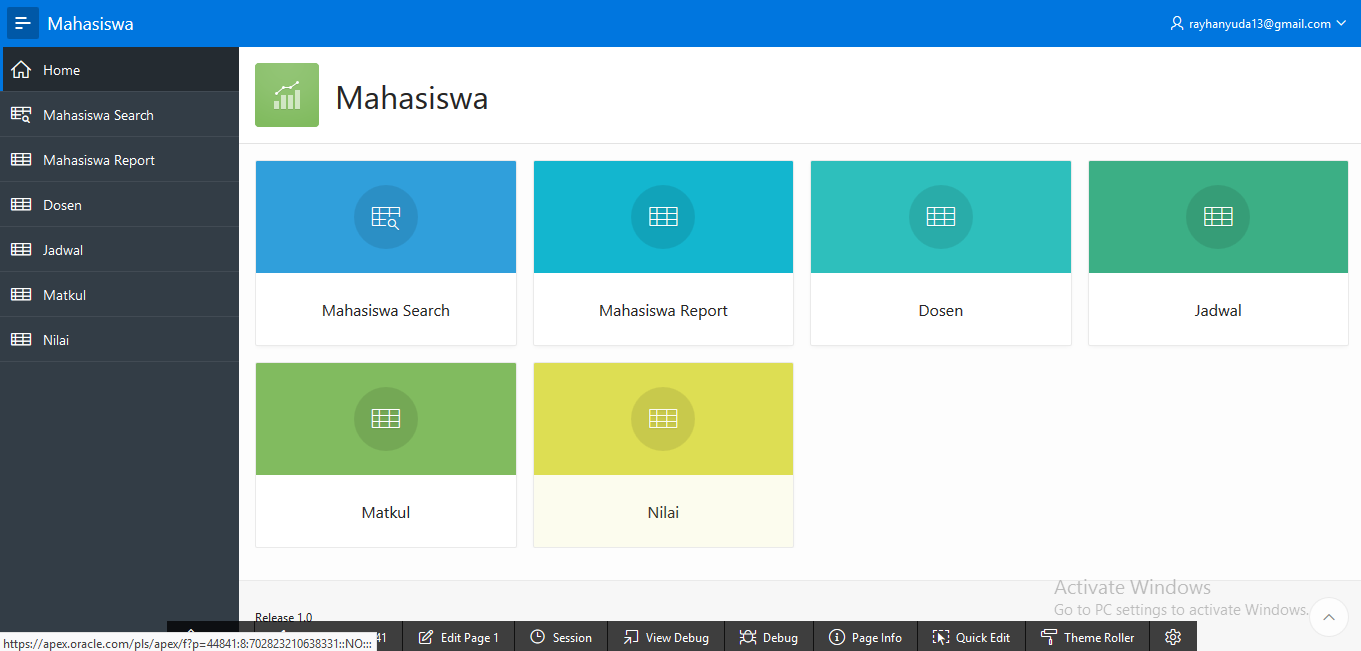
\includegraphics[width=4cm]{gambar/24.png}
\end{figure} 
\end{enumerate}

\chapter*{Email and link}
Email:rayhanyuda13@gmail.com\\
Pass:rayhan1302\\
Link application:https://apex.oracle.com/pls/apex/f?p=44841:1:106557126483270:::::\\
\end{document}